\boxde
\Opensolutionfile{ans}[ans/2D1-2-DEON-3]
\begin{ex}%[2D1Y2-2]
    Cho hàm số $y=f(x)$ có bảng biến thiên. Khẳng định nào sau đây là đúng?
    \begin{center}
        \begin{tikzpicture}
            \tkzTabInit[nocadre=false, lgt=0.7,espcl=2.5,deltacl=0.6]
            {$x$/0.6,$y'$ /0.6, $y$ /3}
            {$-\infty$,$2$,$4$,$+\infty$}
            \tkzTabLine{,+,0,-,0,+}
            \path
            (N13)node[above=0.1cm,fill=white](A){$-\infty$}
            (barycentric cs:N22=2,N23=1)node[fill=white](B){$3$}
            (barycentric cs:N32=1,N33=2)node[fill=white](C){$-2$}
            (N42)node[below=0.1cm,fill=white](D){$+\infty$}
            ;
            \draw[-stealth](A)--(B);
            \draw[-stealth](B)--(C);
            \draw[-stealth] (C)--(D);
        \end{tikzpicture}
    \end{center}
    \choice
    {\True Hàm số đạt cực đại tại $x=2$}
    {Hàm số đạt cực đại tại $x=3$}
    {Hàm số đạt cực đại tại $x=-2$}
    {Hàm số đạt cực đại tại $x=4$}
    \loigiai{
        Dựa vào bảng biến thiên, ta có hàm số đạt cực đại tại $x=2$.}
\end{ex}
\begin{ex}%[2D1Y2-2]
    \immini{Cho hàm số $y=f(x)$ có đồ thị như hình. Mệnh đề nào {\bf đúng}?
        \choice
        {Hàm số có giá trị cực tiểu bằng $2$}
        {Hàm số có giá trị lớn nhất bằng $2$}
        {\True Hàm số đạt cực đại tại $x=0$ và cực tiểu tại $x=2$}
        {Hàm số có ba điểm cực trị}}
    {
        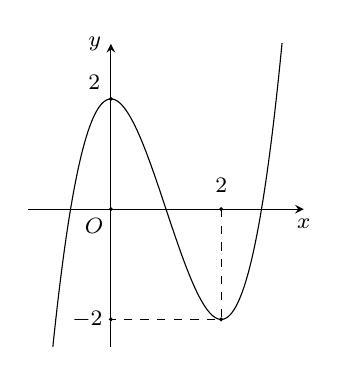
\begin{tikzpicture}[scale=0.7,>=stealth,font=\footnotesize]
            \def\mx{-1.5} \def\max{3.5}
            \def\my{-2.5} \def\may{3}
            \def\hamso(#1,#2){plot [samples=200,smooth,domain=#1:#2](\x,{
                    1*(\x)^3-3*(\x)^2+2
                })}
            \draw[fill=black] (2,-2)circle (.7pt)
            (0,0)circle (.7pt) node[shift={(-135:.3)}]{$O$}
            (2,0)circle (.7pt) node[shift={(90:.3)}]{$2$};
            \foreach \p/\g in {2/135,-2/180}\draw[fill=black] (0,\p)circle (.7pt) node[shift={(\g:.3)}]{$\p$};
            \draw[dashed,thin] (2,0)|-(0,-2);
            %===========================================
            \draw[->] (\mx,0)--(\max,0) node[below] {$x$};
            \draw[->] (0,\my)--(0,\may) node[left] {$y$};
            \clip (\mx,\my) rectangle (\max,\may);
            \draw \hamso(\mx,\max);
    \end{tikzpicture}}
    \loigiai{
        Dựa vào đồ thị hàm số, ta có hàm số đạt cực đại tại $x=0$ và cực tiểu tại $x=2$. }
\end{ex}
\begin{ex}%[2D1Y2-1]
    Hàm số $y=\dfrac{-2x+1}{x-3}$ có bao nhiêu điểm cực trị?
    \choice
    {$1$}
    {\True $0$}
    {$3$}
    {$2$}
    \loigiai{
        Tập xác định $ \mathscr{D}=\mathbb{R}\setminus\{3\}$.\\
        $y'=\dfrac{5}{(x-3)^2}>0$ $\forall x\in\mathbb{R}\setminus\{3\}$.\\
        Suy ra hàm số không có cực trị.}
\end{ex}
\begin{ex}%[2D1B2-1]
    Điểm cực tiểu của đồ thị hàm số $y=x^3-3x+5$ là
    \choice
    {$x=1$}
    {\True $M(1;3)$}
    {$x=-1$}
    {$N(-1;7)$}
    \loigiai{
        Tập xác định $ \mathscr{D}=\mathbb{R}$.\\
        $y'=3x^2-3$, $y'=0\Leftrightarrow x=\pm 1$.\\
        Bảng biến thiên
        \begin{center}
            \begin{tikzpicture}
                \tkzTabInit[nocadre=false, lgt=0.7,espcl=2.5,deltacl=0.6]
                {$x$/0.6,$y'$ /0.6, $y$ /3}
                {$-\infty$,$-1$,$1$,$+\infty$}
                \tkzTabLine{,+,0,-,0,+}
                \path
                (N13)node[above=0.1cm,fill=white](A){$-\infty$}
                (barycentric cs:N22=2,N23=1)node[fill=white](B){$7$}
                (barycentric cs:N32=1,N33=2)node[fill=white](C){$3$}
                (N42)node[below=0.1cm,fill=white](D){$+\infty$}
                ;
                \draw[-stealth](A)--(B);
                \draw[-stealth](B)--(C);
                \draw[-stealth] (C)--(D);
            \end{tikzpicture}
        \end{center}
        Suy ra điểm cực tiểu của đồ thị hàm số $y=x^3-3x+5$ là $M(1;3)$.
    }
\end{ex}
\begin{ex}%[2D1B2-1]
    Tìm điểm cực đại của hàm số $y=x^4-2x^2+2$.
    \choice
    {$(-1;1)$}
    {$x=-1$}
    {$(0;2)$}
    {\True $x=0$}
    \loigiai{
        Tập xác định $ \mathscr{D}=\mathbb{R}$.\\
        $y'=4x^3-4x$, $y'=0\Leftrightarrow \hoac{&x=0\\&x=1\\&x=-1.}$\\
        Bảng biến thiên
        \begin{center}
            \begin{tikzpicture}
                \tkzTabInit[nocadre=false, lgt=0.7,espcl=2.5,deltacl=0.6]
                {$x$/0.6,$y'$ /0.6, $y$ /3}
                {$-\infty$,$-1$,$0$,$1$,$+\infty$}
                \tkzTabLine{,-,0,+,0,-,0,+}
                \path
                (N12)node[below=0.1cm,fill=white](A){$+\infty$}
                (N23)node[above=0.1cm,fill=white](B){$1$}
                (barycentric cs:N32=2,N33=1)node[fill=white](C){$2$}
                (N43)node[above=0.1cm,fill=white](D){$1$}
                (N52)node[below=0.1cm,fill=white](E){$+\infty$}
                ;
                \draw[-stealth](A)--(B);
                \draw[-stealth](B)--(C);
                \draw[-stealth] (C)--(D);
                \draw[-stealth] (D)--(E);
            \end{tikzpicture}
        \end{center}
        Suy ra điểm cực đại của hàm số $y=x^4-2x^2+2$ là $x=0$.
    }
\end{ex}
\begin{ex}%[2D1B2-1]
    Giá trị cực tiểu của hàm số $y=x^3-3x^2-9x+2$ là
    \choice
    {$-20$}
    {$7$}
    {\True $-25$}
    {$3$}
    \loigiai{
        Tập xác định $ \mathscr{D}=\mathbb{R}$.\\
        $y'=3x^2-6x-9$, $y'=0\Leftrightarrow \hoac{&x=-1\\&x=3.}$\\
        Bảng biến thiên
        \begin{center}
            \begin{tikzpicture}
                \tkzTabInit[nocadre=false, lgt=0.7,espcl=2.5,deltacl=0.6]
                {$x$/0.6,$y'$ /0.6, $y$ /3}
                {$-\infty$,$-1$,$3$,$+\infty$}
                \tkzTabLine{,+,0,-,0,+}
                \path
                (N13)node[above=0.1cm,fill=white](A){$-\infty$}
                (barycentric cs:N22=2,N23=1)node[fill=white](B){$7$}
                (barycentric cs:N32=1,N33=2)node[fill=white](C){$-25$}
                (N42)node[below=0.1cm,fill=white](D){$+\infty$}
                ;
                \draw[-stealth](A)--(B);
                \draw[-stealth](B)--(C);
                \draw[-stealth] (C)--(D);
            \end{tikzpicture}
        \end{center}
        Suy ra giá trị cực tiểu của hàm số $y=x^3-3x^2-9x+2$ là $-25$.}
\end{ex}
\begin{ex}%[2D1B2-1]
    Cho hàm số $y=\dfrac{x+1}{x^2+8}$. Mệnh đề nào dưới đây {\bf đúng}?
    \choice
    {\True Cực đại của hàm số bằng $\dfrac{1}{4}$}
    {Cực đại của hàm số bằng $-\dfrac{1}{8}$}
    {Cực đại của hàm số bằng $2$}
    {Cực đại của hàm số bằng $-4$}
    \loigiai{
        Tập xác định $ \mathscr{D}=\mathbb{R}$.\\
        $y'=\dfrac{-x^2-2x+8}{(8+x^2)^2}$, $y'=0\Rightarrow \hoac{&x=2\\&x=-4.}$\\
        Bảng biến thiên
        \begin{center}
            \begin{tikzpicture}
                \tkzTabInit[nocadre=false, lgt=0.7,espcl=2.5,deltacl=0.6]
                {$x$/0.6,$y'$ /0.6, $y$ /3}
                {$-\infty$,$-4$,$2$,$+\infty$}
                \tkzTabLine{,-,0,+,0,-}
                \path
                (N12)node[below=0.1cm,fill=white](A){$+\infty$}
                (barycentric cs:N22=1,N23=2)node[fill=white](B){$-\dfrac{1}{8}$}
                (barycentric cs:N32=2,N33=1)node[fill=white](C){$\dfrac{1}{4}$}
                (N43)node[above=0.1cm,fill=white](D){$-\infty$}
                ;
                \draw[-stealth](A)--(B);
                \draw[-stealth](B)--(C);
                \draw[-stealth] (C)--(D);
            \end{tikzpicture}
        \end{center}
        Suy ra cực đại của hàm số bằng $\dfrac{1}{4}$.
    }
\end{ex}
\begin{ex}%[2D1B2-1]
    Cho hàm số $y=\dfrac{x^2-3x+1}{x}$. Giá trị của tổng $y_\text{CĐ}+y_\text{CT}$ bằng
    \choice
    {\True $-6$}
    {$-1$}
    {$0$}
    {$-5$}
    \loigiai{
        Tập xác định $ \mathscr{D}=\mathbb{R}\setminus\{0\}$.\\
        $y'=\dfrac{x^2-1}{x^2}$, $y'=0\Rightarrow \hoac{&x=1\\&x=-1.}$\\
        Bảng biến thiên
        \begin{center}
            \begin{tikzpicture}
                \tkzTabInit[nocadre=false, lgt=0.7,espcl=2.5,deltacl=0.6]
                {$x$/0.6,$y'$ /0.6, $y$ /3}
                {$-\infty$,$-1$,$0$,$1$,$+\infty$}
                \tkzTabLine{,+,0,-,,-,0,+}
                \path
                (N13)node[above=0.1cm,fill=white](A){$-\infty$}
                (barycentric cs:N22=1,N23=1.2)node[fill=white](B){$-5$}
                (N33)node[above left=0.1cm,fill=white](C){$-\infty$}
                (N32)node[below right=0.1cm,fill=white](C'){$+\infty$}
                (barycentric cs:N42=1.2,N43=1)node[fill=white](D){$-1$}
                (N52)node[below=0.1cm,fill=white](E){$+\infty$}
                ;
                \draw[-stealth](A)--(B);
                \draw[-stealth](B)--(C);
                \draw[-stealth] (C')--(D);
                \draw[-stealth] (D)--(E);
                \draw[double](N31)--(N33);
            \end{tikzpicture}
        \end{center}
        Suy ra $y_\text{CĐ}+y_\text{CT}=-6$.
    }
\end{ex}
\begin{ex}%[2D1B2-1]
    Cho hàm số $y=f(x)$ có đạo hàm $f'(x)=x^2(x^2-4)$, $\forall x \in \mathbb{R}$. Mệnh đề nào đúng?
    \choice
    {\True Hàm số đã cho có $2$ điểm cực trị}
    {Hàm số đã cho đạt cực tiểu tại điểm $x=-2$}
    {Hàm số đã cho đạt cực đại tại điểm $x=2$}
    {Hàm số đã cho có $3$ điểm cực trị}
    \loigiai{
        $f'(x)=0\Leftrightarrow \hoac{&x=0\\&x=2\\&x=-2.}$\\
        Bảng biến thiên
        \begin{center}
            \begin{tikzpicture}
                \tkzTabInit[nocadre=false, lgt=0.7,espcl=2.5,deltacl=0.6]
                {$x$/0.6,$y'$ /0.6, $y$ /3}
                {$-\infty$,$-2$,$0$,$2$,$+\infty$}
                \tkzTabLine{,+,0,-,0,-,0,+}
                \path
                (N13)node[above=0.1cm,fill=white](A){$-\infty$}
                (barycentric cs:N22=2,N23=1)node[fill=white](B){$f(-2)$}

                (barycentric cs:N42=1,N43=2)node[fill=white](C){$f(2)$}
                (N52)node[below=0.1cm,fill=white](D){$+\infty$}
                ;
                \draw[-stealth](A)--(B);
                \draw[-stealth](B)--(C);
                \draw[-stealth] (C)--(D);
            \end{tikzpicture}
        \end{center}
        Suy ra hàm số đã cho đạt cực đại tại điểm $x=-2$, đạt cực tiểu tại điểm $x=2$.\\
        Vậy hàm số đã cho có $2$ điểm cực trị.
    }
\end{ex}
\begin{ex}%[2D1K2-2]
    \immini{Cho hàm số $y=f(x)$ có đồ thị như hình vẽ bên dưới. Hỏi đồ thị hàm số $y=\left|f(x)\right|$ có bao
        nhiêu điểm cực trị?
        \choice
        {\True $5$}
        {$2$}
        {$3$}
        {$4$}}
    {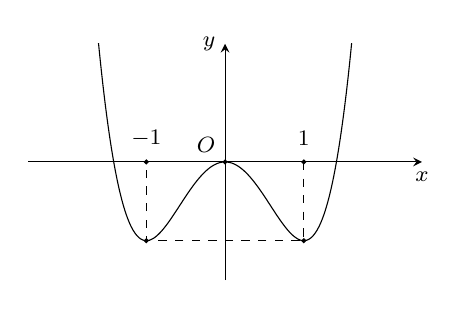
\begin{tikzpicture}[scale=1,>=stealth,font=\footnotesize]
            \def\mx{-2.5} \def\max{2.5}
            \def\my{-1.5} \def\may{1.5}
            \def\hamso(#1,#2){plot [samples=200,smooth,domain=#1:#2](\x,{
                    1*(\x)^4-2*(\x)^2
                })}
            \foreach \p in {-1,1}{
                \draw[fill=black] (\p,0)circle (.7pt) node[shift={(90:.3)}]{$\p$};
                \draw[fill=black] (\p,-1)circle (.7pt);}
            \draw[fill=black] (0,0)circle (.7pt)node [above left] {$O$};
            \draw[dashed,thin] (1,0)|-(0,-1)-|(-1,0);
            %===========================================
            \draw[->] (\mx,0)--(\max,0) node[below] {$x$};
            \draw[->] (0,\my)--(0,\may) node[left] {$y$};
            \clip (\mx,\my) rectangle (\max,\may);
            \draw \hamso(\mx,\max);
    \end{tikzpicture}}
    \loigiai{
        Đồ thị hàm số $y=\left|f(x)\right|$.
        \begin{center}
            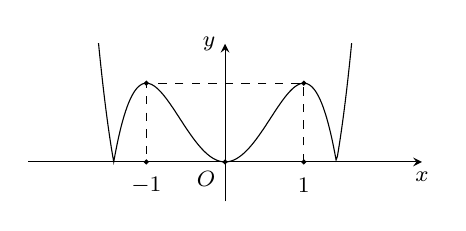
\begin{tikzpicture}[scale=1,>=stealth,font=\footnotesize]
                \def\mx{-2.5} \def\max{2.5}
                \def\my{-0.5} \def\may{1.5}
                \def\f(#1){
                    abs(1*(#1)^4-2*(#1)^2
                    )}
                \foreach \p in {-1,1}{
                    \draw[fill=black] (\p,0)circle (.7pt) node[shift={(-90:.3)}]{$\p$};
                    \draw[fill=black] (\p,1)circle (.7pt);}
                \draw[fill=black] (0,0)circle (.7pt)node [below left] {$O$};
                \draw[dashed,thin] (1,0)|-(0,1)-|(-1,0);
                %===========================================
                \draw[->] (\mx,0)--(\max,0) node[below] {$x$};
                \draw[->] (0,\my)--(0,\may) node[left] {$y$};
                \clip (\mx,\my) rectangle (\max,\may);
                \draw[samples=300] plot[domain=\mx:\max] (\x,{\f(\x)});
            \end{tikzpicture}
        \end{center}
        Suy ra đồ thị hàm số $y=\left|f(x)\right|$ có $5$ cực trị.
    }
\end{ex}
\begin{ex}%[2D1K2-2]
    \immini{Đồ thị hàm số $y=f(x)$ liên tục trên $\mathbb{R}$ và có đồ thị như hình vẽ. Hỏi đồ thị hàm số $y=f\left(|x|\right)$ có tất cả bao nhiêu điểm cực trị?
        \choice
        {$2$}
        {$3$}
        {$4$}
        {$5$}}
    {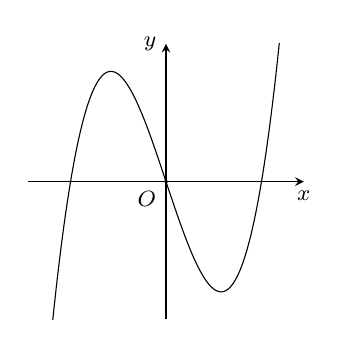
\begin{tikzpicture}[scale=0.7,>=stealth,font=\footnotesize]
            \def\mx{-2.5} \def\max{2.5}
            \def\my{-2.5} \def\may{2.5}
            \def\hamso(#1,#2){plot [samples=200,smooth,domain=#1:#2](\x,{
                    (\x)^3-3*(\x)
                })}
            \draw[fill=black] (0,0)circle (.7pt) node [below left] {$O$};
            %===========================================
            \draw[->] (\mx,0)--(\max,0) node[below] {$x$};
            \draw[->] (0,\my)--(0,\may) node[left] {$y$};
            \clip (\mx,\my) rectangle (\max,\may);
            \draw \hamso(\mx,\max);
    \end{tikzpicture}}
    \loigiai{
        Đồ thị hàm số $y=f\left(|x|\right)$.
        \begin{center}
            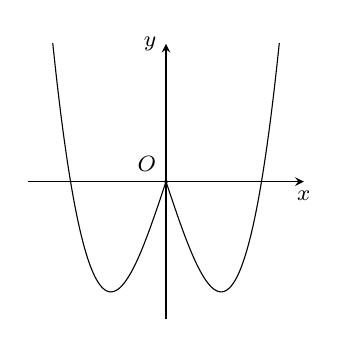
\begin{tikzpicture}[scale=0.7,>=stealth,font=\footnotesize]
                \def\mx{-2.5} \def\max{2.5}
                \def\my{-2.5} \def\may{2.5}
                \def\hamso(#1,#2){plot [samples=200,smooth,domain=#1:#2](\x,{
                        (\x)^3-3*(\x)
                    })}
                \draw[fill=black] (0,0)circle (.7pt) node [above left] {$O$};
                %===========================================
                \draw[->] (\mx,0)--(\max,0) node[below] {$x$};
                \draw[->] (0,\my)--(0,\may) node[left] {$y$};
                \clip (\mx,\my) rectangle (\max,\may);
                \foreach \i in{1,-1}\draw[xscale=\i] \hamso(0,\max);
            \end{tikzpicture}
        \end{center}
        Suy ra đồ thị hàm số $y=f\left(|x|\right)$ có $3$ cực trị.
    }
\end{ex}
\begin{ex}%[2D1K2-1]
    Đồ thị hàm số $y=x^3+3x^2-9x+15$ có hai điểm cực trị $A$, $B$. Độ dài đoạn $AB$ là
    \choice
    {$2\sqrt{65}$}
    {$5\sqrt{55}$}
    {\True $4\sqrt{65}$}
    {$4\sqrt{26}$}
    \loigiai{
        Tập xác định $ \mathscr{D}=\mathbb{R}$.\\
        $y'=3x^2+6x-9$, $y'=0\Leftrightarrow \hoac{&x=1\\&x=-3.}$\\
        Giả sử $A(1;10)$, $B(-3;42)$.\\
        Suy ra $AB=\sqrt{(-3-1)^2+(42-10)^2}=4\sqrt{65}$.
    }
\end{ex}
\begin{ex}%[2D1K2-1]
    Đồ thị hàm số $y=-x^4+2x^2+5$ có ba điểm cực trị là $A$, $B$, $C$. Tìm tọa độ trọng tâm $G$ của tam giác $ABC$.
    \choice
    {$G\left(0; \dfrac{11}{3}\right)$}
    {\True $G\left(0; \dfrac{17}{3}\right)$}
    {$G(0; 4)$}
    {$G\left(1; \dfrac{13}{3}\right)$}
    \loigiai{
        Tập xác định $ \mathscr{D}=\mathbb{R}$.\\
        $y'=-4x^3+4x$, $y'=0\Leftrightarrow \hoac{&x=0\\&x=1\\&x=-1.}$\\
        Giả sử $A(0;5)$, $B(-1;6)$, $C(1;6)$.\\
        Suy ra $G\left(0; \dfrac{17}{3}\right)$.
    }
\end{ex}
\begin{ex}%[2D1K2-1]
    Đồ thị hàm số $y=x^3-3x+2$ có hai điểm cực trị $A$, $B$. Diện tích tam giác $OAB$ bằng
    \choice
    {\True $2$}
    {$\dfrac{1}{2}$}
    {$3$}
    {$4$}
    \loigiai{
        Tập xác định $ \mathscr{D}=\mathbb{R}$.\\
        $y'=3x^2-3$, $y'=0\Leftrightarrow \hoac{&x=1\\&x=-1.}$\\
        Giả sử $A(1;0)$, $B(-1;4)$. Khi đó\\
        $AB=\sqrt{(-1-1)^2+(4-0)^2}=2\sqrt{5}$.\\
        Phương trình đường thẳng $AB$ là $2x+y-2=0$.\\
        $\mathrm{d}(O,AB)=\dfrac{|-2|}{\sqrt{2^2+1^2}}=\dfrac{2}{\sqrt{5}}$.\\
        $S_{OAB}=\dfrac{1}{2}AB\cdot\mathrm{d}(O,AB)=2$.}
\end{ex}
\begin{ex}%[2D1K2-1]
    Goi $A$, $B$, $C$ là ba điểm cực trị của đồ thị hàm số $y=x^4-2x^2+4$. Bán kính đường tròn nội
    tiếp tam giác $ABC$ bằng
    \choice
    {$1$}
    {$1+\sqrt{2}$}
    {\True $\sqrt{2}-1$}
    {$\sqrt{2}$}
    \loigiai{
        Tập xác định $ \mathscr{D}=\mathbb{R}$.\\
        $y'=4x^3-4x$, $y'=0\Leftrightarrow \hoac{&x=0\\&x=1\\&x=-1.}$\\
        Giả sử $A(0;4)$, $B(-1;3)$, $C(1;3)$. Khi đó
        $AB=AC=\sqrt{2}$, $BC=2$.\\
        Suy ra tam giác $ABC$ vuông cân tại $A$.\\
        Vậy bán kính đường tròn nội tiếp tam giác $ABC$ là
        $$r=\dfrac{2S_{ABC}}{AB+BC+CA}=\dfrac{AB\cdot AC}{2+2\sqrt{2}}=\dfrac{2}{2(\sqrt{2}+1)}=\sqrt{2}-1.$$
    }
\end{ex}
\begin{ex}%[2D1B2-1]
    Trong các hàm số sau đây, hàm số nào không có cực trị?
    \choice
    {$y=x^3-3x^2+3$}
    {$y=x^4-x^2+1$}
    {\True $y=x^3+2$}
    {$y=-x^4+3$}
    \loigiai{
        Hàm số $y=x^3+2$ không có cực trị vì $y'=3x^2\ge0$ $\forall x\in \mathbb{R}$.}
\end{ex}
\begin{ex}%[2D1K2-1]
    Đồ thị của hàm số $y=-x^3+3x^2+9x+1$ có hai điểm cực trị $A$ và $B$. Điểm nào dưới đây thuộc đường thẳng $AB$.
    \choice
    {\True $N(1; 12)$}
    {$M(1;-12)$}
    {$P(1;0)$}
    {$Q(0;-1)$}
    \loigiai{
        Tập xác định $ \mathscr{D}=\mathbb{R}$.\\
        $y'=-3x^2+6x+9$, $y'=0\Leftrightarrow \hoac{&x=3\\&x=-1.}$\\
        Giả sử $A(-1;-4)$, $B(3;28)$. Khi đó $\overrightarrow{AB}=(4;32)$.\\
        Phương trình đường thẳng $AB$ là $8x-y+4=0$.\\
        Suy ra $N(1; 12)$ thuộc đường thẳng $AB$.}
\end{ex}
\begin{ex}%[2D1K2-1]
    Tìm điều kiện của hệ số đề đồ thị hàm số bậc ba $y=ax^3+bx^2+cx+d$, $(a \ne 0)$ có hai diềm cực trị nằm về hai phía so với trục tung.
    \choice
    {$a>0$, $b<0$, $c>0$}
    {\True $a\cdot c<0$}
    {$b^2-12ac \ge 0$}
    {$b^2-12ac>0$}
    \loigiai{
        $y'=3ax^2+2bx+c$.\\
        Đồ thị hàm số bậc ba $y=ax^3+bx^2+cx+d$, ($a \ne 0$) có hai diềm cực trị nằm về hai phía so với trục tung khi và chỉ khi phương trình $y'=0$ có hai nghiệm trái dấu hay $a\cdot c<0$.}
\end{ex}
\begin{ex}%[2D1K2-4]
    Cho hàm số $y=x^3-3m^2x+m$. Tìm tham số $m$ để trung điểm của hai điểm cực trị của đồ thị hàm số thuộc $d\colon y=1$.
    \choice
    {$m=\dfrac{1}{3}$}
    {$m=-\dfrac{1}{3}$}
    {\True $m=1$}
    {$m=\dfrac{1}{2}$}
    \loigiai{
        Tập xác định $ \mathscr{D}=\mathbb{R}$.\\$y'=3x^2-3m^2$, $y'=0\Leftrightarrow x=\pm m$.\\
        Hàm số có hai điểm cực trị khi và chỉ khi $m\ne 0$.\\
        Giả sử hai điểm cực trị là $A(m;-2m^2+m)$, $B(-m;2m^2+m)$.\\
        Khi đó trung điểm của hai điểm cực trị là $I(0;m)$. \\
        Theo bài ra $I\in d\Rightarrow m=1$.
    }
\end{ex}
\begin{ex}%[2D1B2-4]
    Tìm các giá trị của tham số $m$ đề hàm số $y=x^3+x^2-(2m+1)x+4$ có đúng hai cực trị?
    \choice
    {$m<\dfrac{4}{3}$}
    {\True $m>-\dfrac{2}{3}$}
    {$m<-\dfrac{2}{3}$}
    {$m>-\dfrac{4}{3}$}
    \loigiai{
        Tập xác định $ \mathscr{D}=\mathbb{R}$.\\$y'=3x^2+2x-(2m+1)$.\\
        Hàm số có hai điểm cực trị khi và chỉ khi $y'=0$ có hai nghiệm phân biệt hay $$\Delta'>0\Leftrightarrow 1+3(2m+1)>0\Leftrightarrow m>-\dfrac{2}{3}.$$
    }
\end{ex}
\begin{ex}%[2D1B2-4]
    Tìm các giá trị của tham số $m$ để hàm số $y=\dfrac{1}{3}x^3-mx^2+(m+2)x+2018$ không có cực trị.
    \choice
    {$m \le-1$}
    {$m \ge 2$}
    {\True $-1 \le m \le 2$}
    {$-1 \le m \le 1$}
    \loigiai{
        Tập xác định $ \mathscr{D}=\mathbb{R}$.\\
        $y'=x^2-2mx+(m+2)$.\\
        Hàm số không có cực trị khi và chỉ khi $y'=0$ không có hai nghiệm phân biệt hay $$\Delta'\le 0\Leftrightarrow m^2-(m+2)\le0\Leftrightarrow -1 \le m \le 2.$$}
\end{ex}
\begin{ex}%[2D1B2-5]
    Tìm các giá trị của tham số $m$ để hàm số $y=x^4-2mx^2+m-1$ có đúng $1$ điểm cực trị.
    \choice
    {\True $m \le 0$}
    {$m>0$}
    {$m \in \mathbb{R}$}
    {$m \in \varnothing$}
    \loigiai{
        Tập xác định $ \mathscr{D}=\mathbb{R}$.\\
        $y'=4x^3-4mx$, $y'=0\Leftrightarrow\hoac{&x=0\\&x^2=m}$ .\\
        Hàm số có $1$ điểm cực trị khi và chỉ khi $y'=0$ đúng một nghiệm hay $m\le0$.}
\end{ex}
\begin{ex}%[2D1B2-5]
    Tìm tất cả các giá trị của tham số $m$ để hàm số $y=(m+1)x^4-mx^2+3$ có ba điểm cực trị.
    \choice
    {$m \in (-\infty;-1) \cup [0;+\infty )$}
    {$m \in (-1; 0)$}
    {$m \in (-\infty;-1] \cup [0;+\infty )$}
    {\True $m \in (-\infty;-1) \cup (0;+\infty )$}
    \loigiai{
        Tập xác định $ \mathscr{D}=\mathbb{R}$.\\
        $y'=4(m+1)x^3-2mx$, $y'=0\Leftrightarrow\hoac{&x=0\\&2(m+1)x^2=m.}$ \\
        Hàm số có ba điểm cực trị khi và chỉ khi $y'=0$ ba nghiệm phân biệt hay $$\hoac{&m+1\ne0\\&\dfrac{m}{2(m+1)}>0}\Leftrightarrow\hoac{&m<-1\\&m>0.}$$
    }
\end{ex}
\begin{ex}%[2D1B2-5]
    Tìm tất cả các tham số $m$ để hàm số $f(x)=x^4+x^3-mx^2$ có ba điểm cực trị.
    \choice
    {$m \in (0;+\infty )$}
    {$m \in (-\infty; 0)$}
    {$m \in \left(-\dfrac{9}{2};+\infty \right)\setminus \{0\}$}
    {\True $m \in \left(-\dfrac{9}{32};+\infty \right)\setminus \{0\}$}
    \loigiai{
        Tập xác định $ \mathscr{D}=\mathbb{R}$.\\
        $y'=4x^3+3x^2-2mx$, $y'=0\Leftrightarrow\hoac{&x=0\\&2x^2+3x-2m=0.\qquad(*)}$ \\
        Hàm số có ba điểm cực trị khi và chỉ khi $y'=0$ ba nghiệm phân biệt khi và chỉ khi $(*)$ hai nghiệm phân biệt khác $0$ hay $$\hoac{&-2m\ne0\\&9+16m>0}\Leftrightarrow\hoac{&m\ne0\\&m>-\dfrac{9}{32}.}$$
    }
\end{ex}
\begin{ex}%[2D1B2-3]
    Tìm tất cả các tham số $m$ đề hàm số $y=x^3-3x^2+mx-2$ đạt cực tiểu tại điểm $x=2$.
    \choice
    {$m>0$}
    {\True $m=0$}
    {$m<0$}
    {$m \ne 0$}
    \loigiai{
        Tập xác định $ \mathscr{D}=\mathbb{R}$.\\
        $y'=3x^2-6x+m$, $y''=6x+6$.\\
        Hàm số $y=x^3-3x^2+mx-2$ đạt cực tiểu tại điểm $x=2$ suy ra $y'(2)=0\Leftrightarrow m=0$.\\
        Với $m=0$ ta có $y''(2)=18>0$.\\
        Suy ra hàm số đạt cực tiểu tại điểm $x=2$.\\
        Vậy $m=0$ thỏa mãn đề bài.
    }
\end{ex}
\begin{ex}%[2D1K2-3]
    Tìm các tham số $m$ để hàm số $f(x)=x^3-3mx^2+3(m^2-1)x$ đạt cực đại tại $x=1$.
    \choice
    {$m=0$}
    {$m \in \mathbb{R}\setminus \{0; 2\}$}
    {$m \in \{0; 2\}$}
    {\True $m=2$}
    \loigiai{
        Tập xác định $ \mathscr{D}=\mathbb{R}$.\\
        $y'=3x^2-6mx+3(m^2-1)$, $y''=6x-6m$.\\
        Hàm số $f(x)=x^3-3mx^2+3(m^2-1)x$ đạt cực tiểu tại điểm $x=1$ suy ra $$y'(1)=0\Leftrightarrow 3-6m+3m^2-3=0\Leftrightarrow\hoac{&m=0\\&m=2.}$$\\
        Với $m=0$ ta có $y''=6x\Rightarrow y''(1)=6>0$.\\
        Suy ra hàm số đạt cực tiểu tại điểm $x=1$ (Không thỏa mãn đề bài).\\
        Với $m=2$ ta có $y''=6x-12\Rightarrow y''(1)=-6<0$.\\
        Suy ra hàm số đạt cực tiểu tại điểm $x=1$ (thỏa mãn đề bài).\\
        Vậy $m=2$ thỏa mãn đề bài.}
\end{ex}
\begin{ex}%[2D1K2-4]
    Tìm tất cả các giá trị của tham số $m$ đế đồ thị hàm số $y=\dfrac{1}{3}x^3+x^2+(m-1)x+2$ có hai điểm cực trị đều nằm bên trái trục tung.
    \choice
    {\True $1<m<2$}
    {$m>1$}
    {$m<2$}
    {$m<1$}
    \loigiai{
        Tập xác định $ \mathscr{D}=\mathbb{R}$.\\
        $y'=x^2+2x+(m-1)$.\\
        Đồ thị hàm số $y=\dfrac{1}{3}x^3+x^2+(m-1)x+2$ có hai điểm cực trị đều nằm bên trái trục tung khi và chỉ khi $y'=0$ có hai nghiệm âm phân biệt hay $$\heva{&\Delta'>0\\&S<0\\&P>0}\Leftrightarrow\heva{&1-(m-1)>0\\&-2<0&\text{(luôn đúng)}\\&m-1>0}\Leftrightarrow\heva{&m<2\\&m>1.}$$
    }
\end{ex}
\begin{ex}%[2D1K2-4]
    Biết rằng có hai giá trị của tham số thực $m$ để hàm số $y=x^3-3x^2+m^2+2m$ đạt giá trị cực
    tiểu bằng $-4$. Tính tổng $S$ của hai giá trị $m$ đó.
    \choice
    {$S=1$}
    {\True $S=-2$}
    {$S=3$}
    {$S=5$}
    \loigiai{
        Tập xác định $ \mathscr{D}=\mathbb{R}$.\\
        $y'=3x^2-6x$, $y'=0\Leftrightarrow\hoac{&x=0\\&x=2.}$\\
        Bảng biến thiên
        \begin{center}
            \begin{tikzpicture}
                \tkzTabInit[nocadre=false, lgt=0.7,espcl=2.5,deltacl=0.6]
                {$x$/0.6,$y'$ /0.6, $y$ /3}
                {$-\infty$,$0$,$2$,$+\infty$}
                \tkzTabLine{,+,0,-,0,+}
                \path
                (N13)node[above=0.1cm,fill=white](A){$-\infty$}
                (barycentric cs:N22=2,N23=1)node[fill=white](B){$m^2+2m$}
                (barycentric cs:N32=1,N33=2)node[fill=white](C){$-4+m^2+2m$}
                (N42)node[below=0.1cm,fill=white](D){$+\infty$}
                ;
                \draw[-stealth](A)--(B);
                \draw[-stealth](B)--(C);
                \draw[-stealth] (C)--(D);
            \end{tikzpicture}
        \end{center}
        Theo bài ra ta có $-4+m^2+2m=-4\Leftrightarrow\hoac{&m=0\\&m=-2.}$\\
        Vậy $S=-2$.
    }
\end{ex}
\begin{ex}%[2D1K2-5]
    Tìm tất cả các giá trị thực của tham số $m$ để đồ thị hàm số $y=x^4-4mx^2+3m-2$ có ba điểm cực trị tạo thành một tam giác nhận $G\left(0;-\dfrac{5}{3}\right)$ làm trọng tâm.
    \choice
    {$m=1$}
    {$m=8$}
    {\True $m=1$ hoặc $m=\dfrac{1}{8}$}
    {$m=\dfrac{1}{8}$}
    \loigiai{
        Tập xác định $ \mathscr{D}=\mathbb{R}$.\\
        $y'=4x^3-8mx$, $y'=0\Leftrightarrow\hoac{&x=0\\&x^2=2m.}$\\
        Đồ thị hàm số $y=x^4-4mx^2+3m-2$ có ba điểm cực trị khi và chỉ khi $y'=0$ có 3 nghiệm phân biệt hay $m>0$.\\
        Giả sử ba điểm cực trị là $A(0;3m-2)$, $B(\sqrt{2m};-4m^2+3m-2)$, $C(-\sqrt{2m};-4m^2+3m-2)$.\\
        Theo bài ra ta có $3m-2+2(-4m^2+3m-2)=-5\Leftrightarrow -8m^2+9m-1=0\Leftrightarrow \hoac{&m=1\\&m=\dfrac{1}{8}.}$
    }
\end{ex}
\begin{ex}%[2D1K2-4]
    Tìm các tham số $m$ để hàm số $y=\dfrac{1}{3}x^3-mx^2+(m^2+m-1)x+1$ đạt cực trị tại hai điểm $x_1$, $x_2$ thỏa mãn $|x_1+x_2|=4$.
    \choice
    {$m=2$}
    {$m\in \varnothing$}
    {\True $m=-2$}
    {$m= \pm 2$}
    \loigiai{
        Tập xác định $ \mathscr{D}=\mathbb{R}$.\\
        $y'=x^2-2mx+(m^2+m-1)$.\\
        Hàm số $y=\dfrac{1}{3}x^3-mx^2+(m^2+m-1)x+1$ đạt cực trị tại hai điểm $x_1$, $x_2$ khi và chỉ khi $y'=0$ có hai nghiệm phân biệt hay
        $$\Delta'>0\Leftrightarrow m^2-(m^2+m-1)>0\Leftrightarrow m<1.$$
        Theo bài ra ta có $|x_1+x_2|=4\Leftrightarrow |-2m|=4\Leftrightarrow \hoac{&m=2&\text{(loại)}\\&m=-2&\text{(nhận)}.}$}
\end{ex}
\begin{ex}%[2D1K2-2]
    \immini{Cho hàm số bậc bốn $y=f(x)$ có đồ thị hình vẽ bên. Số điểm cực trị của hàm số $g(x)=f(x^3-3x)$ là
        \choice
        {$7$}
        {\True $9$}
        {$11$}
        {$5$}}
    {
        % Đồ thị hàm y=ax^3+bx^2+cx+d. Nếu hệ số lớn cần điều chỉnh hệ trục, vùng lưới, domain và lệnh \clip
        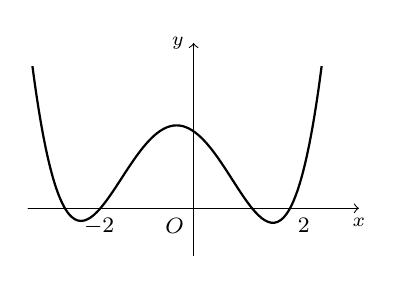
\begin{tikzpicture}[=>stealth,line join=round,line cap=round, font=\footnotesize,scale=.6]
            \def\a{0.12} % Hệ số a phải khác 0
            \def\b{0.17}
            \def\c{-0.9}
            \def\d{-0.69}
            \def\e{1.63}
            %\draw[color=gray,dash pattern=on 1pt off 1pt,xstep=1.0cm,ystep=1.0cm] (-5.2,-5.2) grid (5.2,5.2);
            \draw[->] (-3.5,0) -- (3.5,0)node[below]{\scriptsize $x$};
            \draw[->] (0,-1) -- (0,3.5) node[left] {\scriptsize $y$};
            \draw (0,0)node[below left]{$O$}(-2,0)node[below]{$-2$}(2,0)node[below right]{$2$};
            \clip (-3.5,-1)rectangle(3,3);
            \draw[thick,samples=150,smooth,domain=-5:5] plot(\x,{\a*(\x)^4+(\b)*(\x)^3+(\c)*(\x)^2+(\d)*\x+(\e)});
        \end{tikzpicture}
    }
    \loigiai{
        Ta có $g'(x)=(3x^2-3)\cdot f'(x^3-3x)=0\Leftrightarrow\hoac{&3x^2-3=0\\&f'(x^3-3x)=0}\Leftrightarrow\hoac{&x=\pm 1\\&x^3-3x=a& a\in (-3;-2)\\&x^3-3x=b& b\in (-2;0)\\&x^3-3x=c& c\in (1;2).}$\\
        Bảng biến thiên của hàm số $y=x^3-3x$
        \begin{center}
            
\begin{tikzpicture}[>=stealth]
                \tkzTabInit[nocadre=false,lgt=1,espcl=2,deltacl=0.5]{$x$/.7 ,$y'$/.7,$y$/2}
                {$-\infty$ , $-1$ , $1$ , $+\infty$}
                \tkzTabLine{ , + , $0$ , - , $0$ , + , }
                \tkzTabVar{-/$-\infty$ , +/$2$ , -/$-2$ , +/$+\infty$}

            \end{tikzpicture}
        \end{center}
        \begin{itemize}
            \item Phương trình $x^3-3x=a$ với $a\in (-3;-2)$ có $1$ nghiệm.
            \item Phương trình $x^3-3x=b$ với $b\in (-2;0)$ có $3$ nghiệm.
            \item Phương trình $x^3-3x=c$ với $c\in (1;2)$ có $3$ nghiệm.
        \end{itemize}
        Vậy hàm số $g(x)$ có $9$ điểm cực trị.
    }
\end{ex}
\begin{ex}%[2D1K2-6]
    \immini{Cho hàm số $f=f(x)$ có đạo hàm trên $\mathbb{R}$. Đồ thị hàm số $y=f'(x)$ như hình vẽ. Tìm tất cả các giá trị của tham số $m$ để hàm số $y=f(x)-mx$ có $3$ điểm cực trị?
        \choice
        {\True $0<m<4$}
        {$0\le m\le4$}
        {$m>4$}
        {$m<0$}}
    {	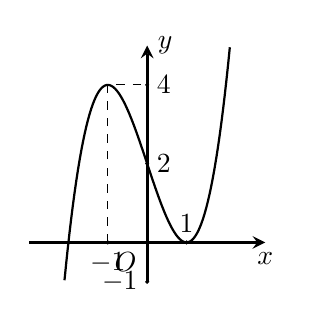
\begin{tikzpicture}[>=stealth,scale=0.5]
            \draw[->,line width = 1pt] (-3,0)--(0,0) node[below left]{$O$}--(3,0) node[below]{$x$};
            \draw[->,line width = 1pt] (0,-1) --(0,5) node[right]{$y$};
            \draw (-1,0) node[below]{$-1$} circle (1pt);
            \draw (0,2) node[right]{$2$} circle (1pt);
            \draw (0,4) node[right]{$4$} circle (1pt);
            \draw (0,-1) node[left]{$-1$} circle (1pt);
            \draw (1,0) node[above]{$1$} circle (1pt);
            \draw [thick, domain=-2.1:2.1, samples=100] %
            plot (\x, {(\x)^3-3*(\x)+2});
            \draw [dashed] (-1,0)--(-1,4)--(0,4);
    \end{tikzpicture}}
    \loigiai{
        Đặt $y=g(x)=f(x)-mx \Rightarrow g'(x)=f'(x)-m$.\\
        Hàm số $g(x)$ có $3$ điểm cực trị khi và chỉ khi phương trình $g'(x)=0$ có $3$ nghiệm phân biệt.\\
        Suy ra $0<m<4$.
    }
\end{ex}
\begin{ex}%[2D1K2-2]
    \immini{Cho hàm số $y=f(x)$ có đạo hàm trên $\mathbb{R}$, $f(-2)=0$. Biết  hàm $y=f'(x)$ có đồ thị như hình vẽ bên. Số điểm cực tiểu của hàm  số $y=g(x)=\left|4f\left(x \right)-x^2+4  \right| $  là
        \choice
        {$1$}
        {\True $3$}
        {$4$}
        {$2$}}{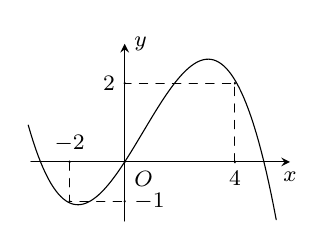
\begin{tikzpicture}[>=stealth,line join=round,line cap=round,font=\footnotesize,scale=.5]
            \begin{scope}[xscale=0.7]
                \draw[->] (-3.4,0)--(6,0)node[below]{$x$};
                \draw[->](0,-1.5)--(0,3)node[right]{$y$};
                \draw[domain=-3.5:5.5,samples=100] plot (\x,{-.07*(\x)^3+.14*(\x)^2+ 1.08*(\x) });
                \draw[dashed] (-2,0)|-(0,-1) (4,0)|-(0,2);
                \fill (-2,0)circle(0.04)node[above]{$-2$}(-2,-1)circle(0.04)
                (4,0)circle(0.04)node[below]{$4$}(4,2)circle(0.04)
                (0,-1)circle(0.04)node[ right]{$-1$}
                (0,2)circle(0.04)node[left]{$2$}
                (0,0)circle(0.04)node[below right]{$O$};
            \end{scope}
    \end{tikzpicture}}
    \loigiai{
        \immini{Đặt $h(x)=4f\left(x \right)-x^2+4$, ta có $h'(x)=4f'(x)-2x$;
            \[h'(x)=0\Leftrightarrow 4f'(x)-2x=0\Leftrightarrow f'(x)=\dfrac{x}{2}.\]
            Vẽ đồ thị của hàm số $y=f'(x)$ và $y=\dfrac{x}{2}$ trên cùng một hệ trục tọa độ, ta được hình vẽ bên.\\
            Dựa vào đồ thị ta có phương trình $f'(x)=\dfrac{x}{2}$ có $3$ nghiệm phân biệt là $-2$, $0$, $4$ và vị trí tương đối giữa hai đồ thị ta suy ra bảng biến thiên của $h(x)$ như sau}{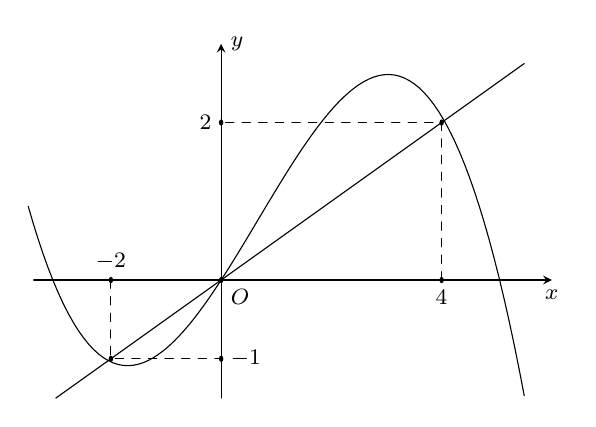
\begin{tikzpicture}[>=stealth,line join=round,line cap=round,font=\footnotesize,scale=1]
                \begin{scope}[xscale=0.7]
                    \draw[->] (-3.4,0)--(6,0)node[below]{$x$};
                    \draw[->](0,-1.5)--(0,3)node[right]{$y$};
                    \draw[domain=-3.5:5.5,samples=100] plot (\x,{-.07*(\x)^3+.14*(\x)^2+ 1.08*(\x) });
                    \draw[domain=-3:5.5,samples=100] plot (\x,{.5*\x});
                    \draw[dashed] (-2,0)|-(0,-1) (4,0)|-(0,2);
                    \fill (-2,0)circle(0.04)node[above]{$-2$}(-2,-1)circle(0.04)
                    (4,0)circle(0.04)node[below]{$4$}(4,2)circle(0.04)
                    (0,-1)circle(0.04)node[ right]{$-1$}
                    (0,2)circle(0.04)node[left]{$2$}
                    (0,0)circle(0.04)node[below right]{$O$};
                \end{scope}
        \end{tikzpicture}}
        \begin{center}
            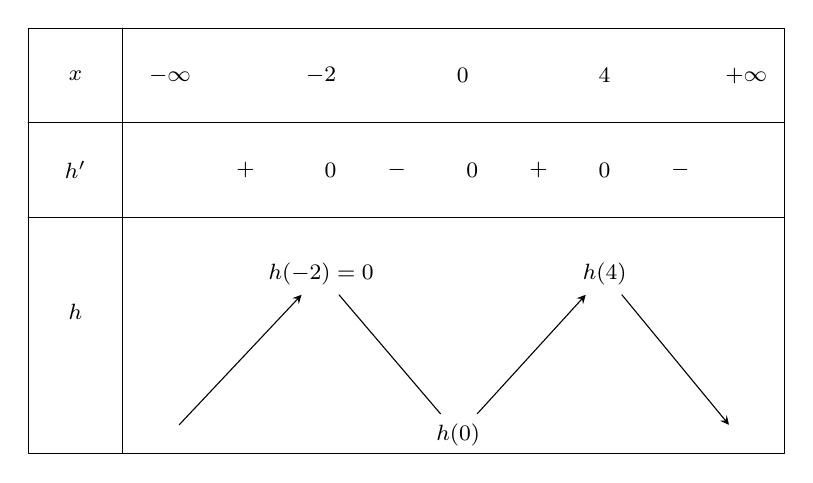
\begin{tikzpicture}[>=stealth,line join=round,line cap=round,font=\footnotesize,scale=1.2]
                \def\a{8}\def\b{4.5}
                \begin{scope}[shift={(-.5,0.5)}]
                    \draw
                    (0,0)rectangle+(\a,-\b)
                    ++(0,-1)--+(0:\a)
                    ++(0,-1)--+(0:\a)
                    (0,0)++(1,0)--+(-90:\b)
                    ;
                \end{scope}
                \path (0,0)node{$x$}++(0:1)node{$-\infty$}++(0:1.6)node{$-2$}++(0:1.5)node{$0$}++(0:1.5)node{$4$}++(0:1.5)node{$+\infty$}
                (0,-1)node{$h'$}++(0:1)node{}++(0:.8)node{$+$}++(0:0.9)node{$0$}++(0:.7)node{$-$}++(0:0.8)node{$0$}++(0:.7)node{$+$}++(0:0.7)node{$0$}++(0:0.8)node{$-$}
                (0,-2.5)node{$h$}
                (1,-3.8)node (A){}
                (2.6,-2.1)node (B){$h(-2)=0$}
                (4.05,-3.8)node (C){$h(0)$}
                (5.6,-2.1)node (D){$h(4)$}
                (7,-3.8)node (E){}
                ;
                \draw[->](A)--(B);
                \draw(B)--(C);
                \draw[->](C)--(D);
                \draw[->](D)--(E);
            \end{tikzpicture}
        \end{center}
        Từ đồ thị hàm số $y=f'(x)$ và $y=\dfrac{x}{2}$, suy ra diện tích giới hạn bởi đồ thị hàm số $y=f'(x)$, $y=\dfrac{x}{2}$ là
        \[\heva{&S_1=\displaystyle\int\limits_{-2}^{0}\left| h'(x)\right| \mathrm{\,d}x=h(-2)-h(0)\\&S_2=\displaystyle\int\limits_{0}^{4}\left| h'(x)\right| \mathrm{\,d}x=h(4)-h(0).}\]
        Từ đồ thị hai hàm số  ta có $S_2>S_1$, suy ra $h(4)>h(-2)>0$.\\
        Do đó, phương trình $4f(x)-x^2+4=0$ có $3$ nghiệm phân biệt là $-2$, $a$, $b$, trong đó $0<a<4<b$.\\
        Vậy $y=g(x)=\left|4f\left(x \right)-x^2+4  \right| $ có $3$ điểm cực tiểu là $-2$, $a$, $b$.
    }
\end{ex}
\begin{ex}%[2D1K2-6]
    Có bao nhiêu giá trị nguyên của tham số $m$ để hàm số $y=\vert3x^4-4x^3-12x^2+m\vert$ có $7$ điểm cực trị?
    \choice
    {$3$}
    {\True $4$}
    {$5$}
    {$5$}
    \loigiai{
        Đặt $f(x)= 3x^4 -4x^3 -12x^2 +m \Rightarrow f'(x)= 12x^3 -12x^2 -24x$. \\
        $\Rightarrow f'(x)=0 \Leftrightarrow \hoac{&x=0\\&x=-1\\&x=2.}$ \\
        Ta có bảng biến thiên của hàm số $y=f(x)$
        \begin{center}
            
\begin{tikzpicture}
                \tkzTabInit[nocadre=false,lgt=1.2,espcl=2.3]
                {$x$ /0.6,$f'(x)$ /0.6,$f(x)$ /2}
                {$-\infty$,$-1$,$0$,$2$,$+\infty$}
                \tkzTabLine{,-,$0$,+,$0$,-,$0$,+,}
                \tkzTabVar{+/$+\infty$, -/$m-5$,+/$m$,-/$m-32$,+/$+\infty$}
            \end{tikzpicture}
        \end{center}
        Ta thấy $m-32<m-5$, hàm số $y=f(x)$ có $3$ điểm cực trị. \\
        Suy ra hàm số $y=\left| f(x)\right| $ có $7$ điểm cực trị khi và chỉ khi phương trình $f(x)=0 $ có $7-3=4$ nghiệm phân biệt, không trùng với điểm cực trị của hàm số $y=f(x)$.\\
        Từ bảng biến thiên, ta suy ra $m-5<0<m\Leftrightarrow 0<m<5$.\\
        Vì $m$ là số nguyên nên $m\in\{1;2;3;4\}$. Vậy có $4$ giạ trị nguyên của $m$.
    }
\end{ex}
\begin{ex}%[2D1G2-6]
    Cho hàm bậc bốn $y=f(x)$ có đồ thị như hình vẽ dưới đây. Số điểm cực trị của hàm số $g(x)=f\left(x^4-4\vert x\vert\right)$ là
    \begin{center}
        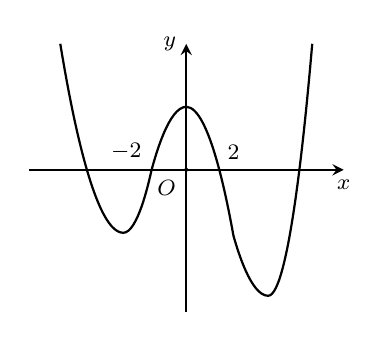
\begin{tikzpicture}[>=stealth,x=1.0cm,y=1.0cm,thick, scale=0.4]
            \draw[->] (-5,0) -- (5,0) node[below] {\footnotesize $x$};
            \draw[->] (0,-4.5) -- (0,4) node[left] {\footnotesize $y$};
            \draw (0,0) node[below left] {\footnotesize $O$} circle (1pt);
            \draw[smooth](-1.1,0) parabola bend (-2,-2)(-4,4);
            \draw(-1.1,0) parabola bend (0,2)(1.5,-2.1);
            \draw[smooth](1.5,-2.1) parabola bend (2.6,-4)(4,4);
            \draw (1.5,0) node[above] {\footnotesize $2$};
            \draw (-1.1,0) node[above left] {\footnotesize $-2$};
        \end{tikzpicture}
    \end{center}
    \choice
    {$5$}
    {$3$}
    {$7$}
    {\True $11$}
    \loigiai{
        Đặt $g(x)=f(x^4-4x)\Rightarrow g'(x)=f'(x^4-4x)\cdot(4x^3-4)=4(x^3-1)f'(x^4-4x)$.\\
        Suy ra $g'(x)=0\Leftrightarrow \hoac{&x^3-1=0\\&f'(x^4-4x)=0.}$\\
        \begin{itemize}
            \item $x^3-1=0\Leftrightarrow x=1$.
            \item $f'(x^4-4x)=0\Leftrightarrow \hoac{&x^4-4x=-2\\&x^4-4x=2\\&x^4-4x=a\quad(a<-2)\\&x^4-4x=b\quad(b>2).}$
            \begin{center}
                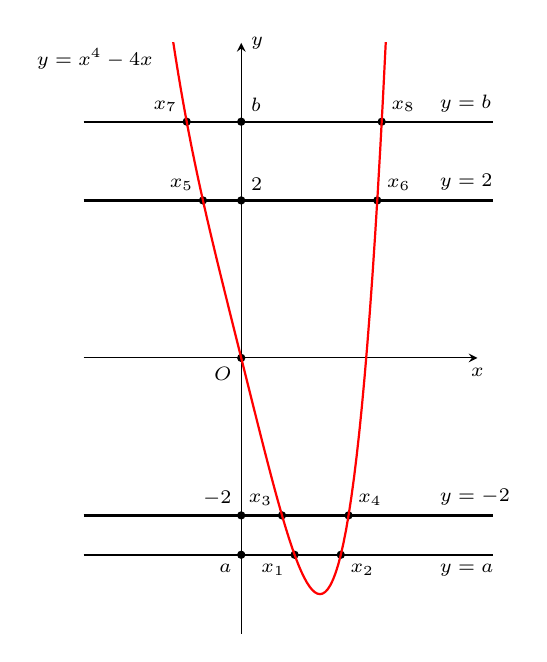
\begin{tikzpicture}[>=stealth,x=1.0cm,y=1.0cm,scale=1]
                    \draw[->] (-2,0)--(3,0) node[below] {\scriptsize $x$};
                    \draw[->] (0,-3.5) --(0,4) node[right] {\scriptsize $y$};
                    \draw [thick, domain=-2:3.2, samples=100] %
                    plot (\x, {0*(\x)+2});
                    \draw [thick, domain=-2:3.2, samples=100] %
                    plot (\x, {0*(\x)-2});
                    \draw [thick, domain=-2:3.2, samples=100] %
                    plot (\x, {0*(\x)+3});
                    \draw [thick, domain=-2:3.2, samples=100] %
                    plot (\x, {0*(\x)-2.5});
                    \draw
                    (0,0)node[below left]{\scriptsize $O$}
                    (0,2)node[above right]{\scriptsize $2$}
                    (0,-2)node[above left]{\scriptsize $-2$}
                    (0,-2.5)node[below left]{\scriptsize $a$}
                    (0,3)node[above right]{\scriptsize $b$}
                    (-1,3.8) node[left]{\scriptsize $y=x^4-4x$}
                    (2.4,2) node[above right]{\scriptsize $y=2$}
                    (2.4,-2) node[above right]{\scriptsize $y=-2$}
                    (2.4,-2.5) node[below right]{\scriptsize $y=a$}
                    (2.4,3) node[above right]{\scriptsize $y=b$}
                    (-0.6925,3) node[above left]{\scriptsize $x_7$}
                    (-0.4860,2) node[above left]{\scriptsize $x_5$}
                    (0.5180,-2) node[above left]{\scriptsize $x_3$}
                    (0.6777,-2.5) node[below left]{\scriptsize $x_1$}
                    (1.2648,-2.5) node[below right]{\scriptsize $x_2$}
                    (1.3631,-2) node[above right]{\scriptsize $x_4$}
                    (1.7278,2) node[above right]{\scriptsize $x_6$}
                    (1.7844,3) node[above right]{\scriptsize $x_8$};
                    \fill[black]
                    (0,0) circle(1.5pt)	(0,3) circle(1.5pt)
                    (0,-2.5) circle(1.5pt)	(0,2) circle(1.5pt)
                    (0,-2) circle(1.5pt)	(-0.6925,3) circle(1.5pt)
                    (-0.4860,2) circle(1.5pt)	(-0.6925,3) circle(1.5pt)
                    (0.5180,-2)  circle(1.5pt)	(0.6777,-2.5) circle(1.5pt)
                    (1.2648,-2.5) circle(1.5pt)	(1.3631,-2)  circle(1.5pt)
                    (1.7278,2)  circle(1.5pt)	(1.7844,3)  circle(1.5pt);
                    \clip (-1,-3.3)rectangle(2,4);
                    \draw [thick,color=red, domain=-1.2:2.1, samples=100] %
                    plot (\x, {(\x)^4-4*(\x)});
                \end{tikzpicture}
            \end{center}
            \begin{itemize}
                \item Phương trình $x^4-4x=a$ có $2$ nghiệm $x_1$, $x_2$ với $x_1<x_2$.
                \item Phương trình $x^4-4x=-2$ có $2$ nghiệm $x_3$, $x_4$ với $x_3<x_4$.
                \item Phương trình $x^4-4x=2$ có $2$ nghiệm $x_5$, $x_6$ với $x_5<x_6$.
                \item Phương trình $x^4-4x=b$ có $2$ nghiệm $x_7$, $x_8$ với $x_7<x_8$.
            \end{itemize}
        \end{itemize}
        Bảng biến thiên
        \begin{center}
            
\begin{tikzpicture}
                \tkzTabInit[nocadre=false,lgt=2.5,espcl=1.3,deltacl=0.5]
                {$x$ /0.7,$x^3-1$ /0.7,$f'(x^4-4x)$ /0.7,$g'(x)$ /0.7,$g(x)$ /2}
                {$-\infty$,$x_7$,$x_5$,$x_3$,$x_1$,$1$,$x_2$,$x_4$, $x_6$, $x_8$,$+\infty$}
                \tkzTabLine{,-,|,-,|,-,|,-,|,-,$0$,+,|,+,|,+,|,+,|,+,}
                \tkzTabLine{,-,$0$,-,$0$,-,$0$,-,$0$,-,|,+,$0$,+,$0$,+,$0$,+,$0$,+,}
                \tkzTabLine{,-,$0$,-,$0$,-,$0$,-,$0$,-,$0$,+,$0$,+,$0$,+,$0$,+,$0$,+,}
                \tkzTabVar{+/,-/,+/,-/,+/,-/,+/,-/,+/,-/,+/}
            \end{tikzpicture}
        \end{center}
        Từ bảng biến thiên suy ra hàm số $y=g(x)$ có $5$ điểm cực trị ứng với $x>0$ nên hàm số $y=f(|x|^4-4|x|)$ có $11$ điểm cực trị.

    }
\end{ex}
\Closesolutionfile{ans}
%\indapan{10}{ans/2D1-2-DEON-1}